% --- PAGE 1 ---
\begin{figure}[htbp]
    \centering

    \begin{subfigure}{\textwidth}
        \centering
        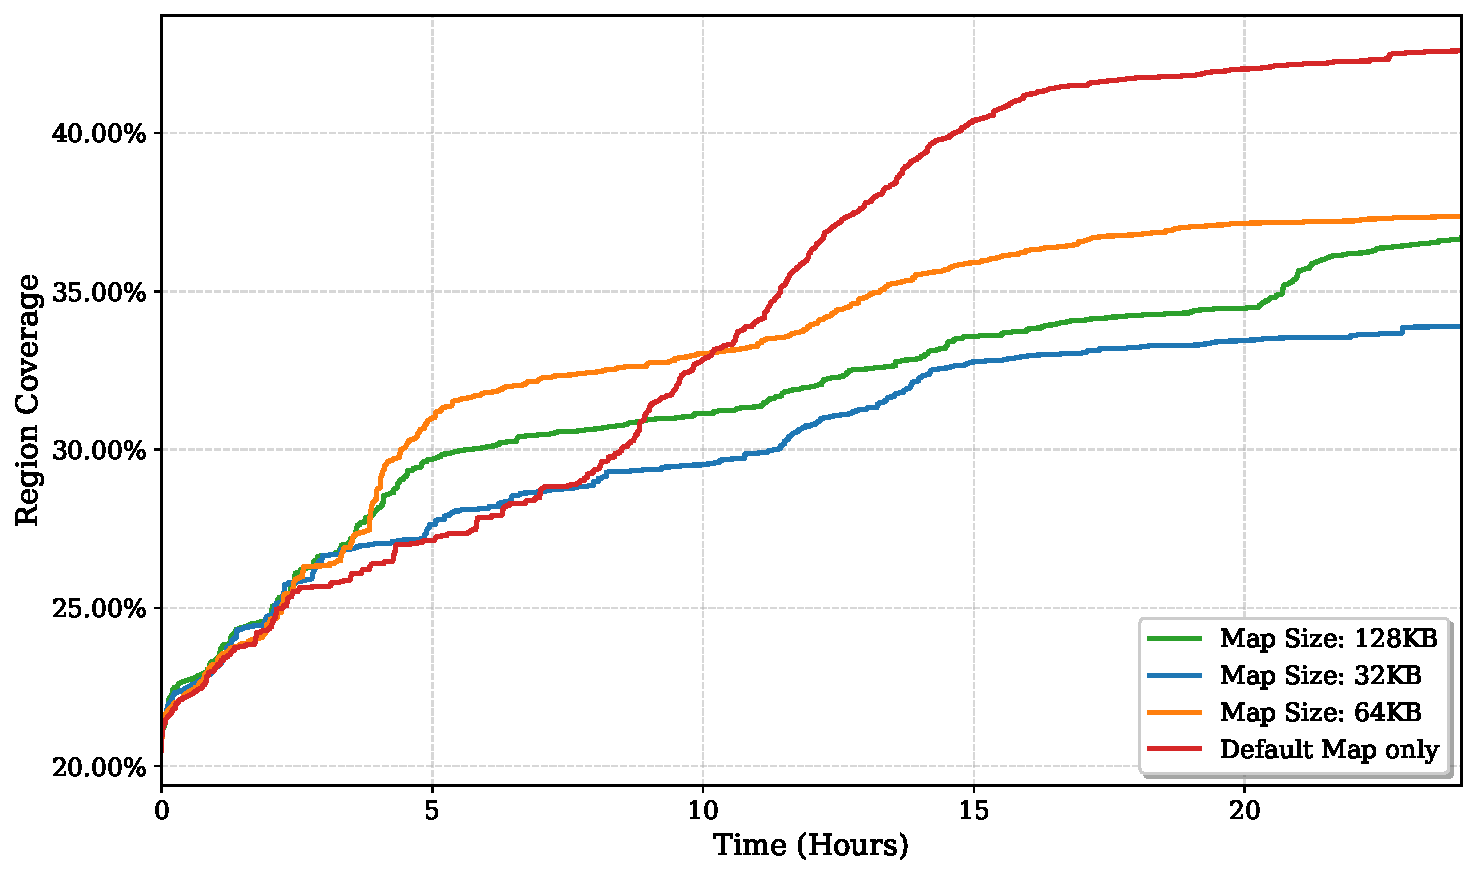
\includegraphics[width=0.85\linewidth]{imgs/eval/coverage_plot_mruby.pdf}
        \caption{mruby}
        \label{fig:plot_mruby}
    \end{subfigure}

    \vspace{2em} 

    \begin{subfigure}{\textwidth}
        \centering
        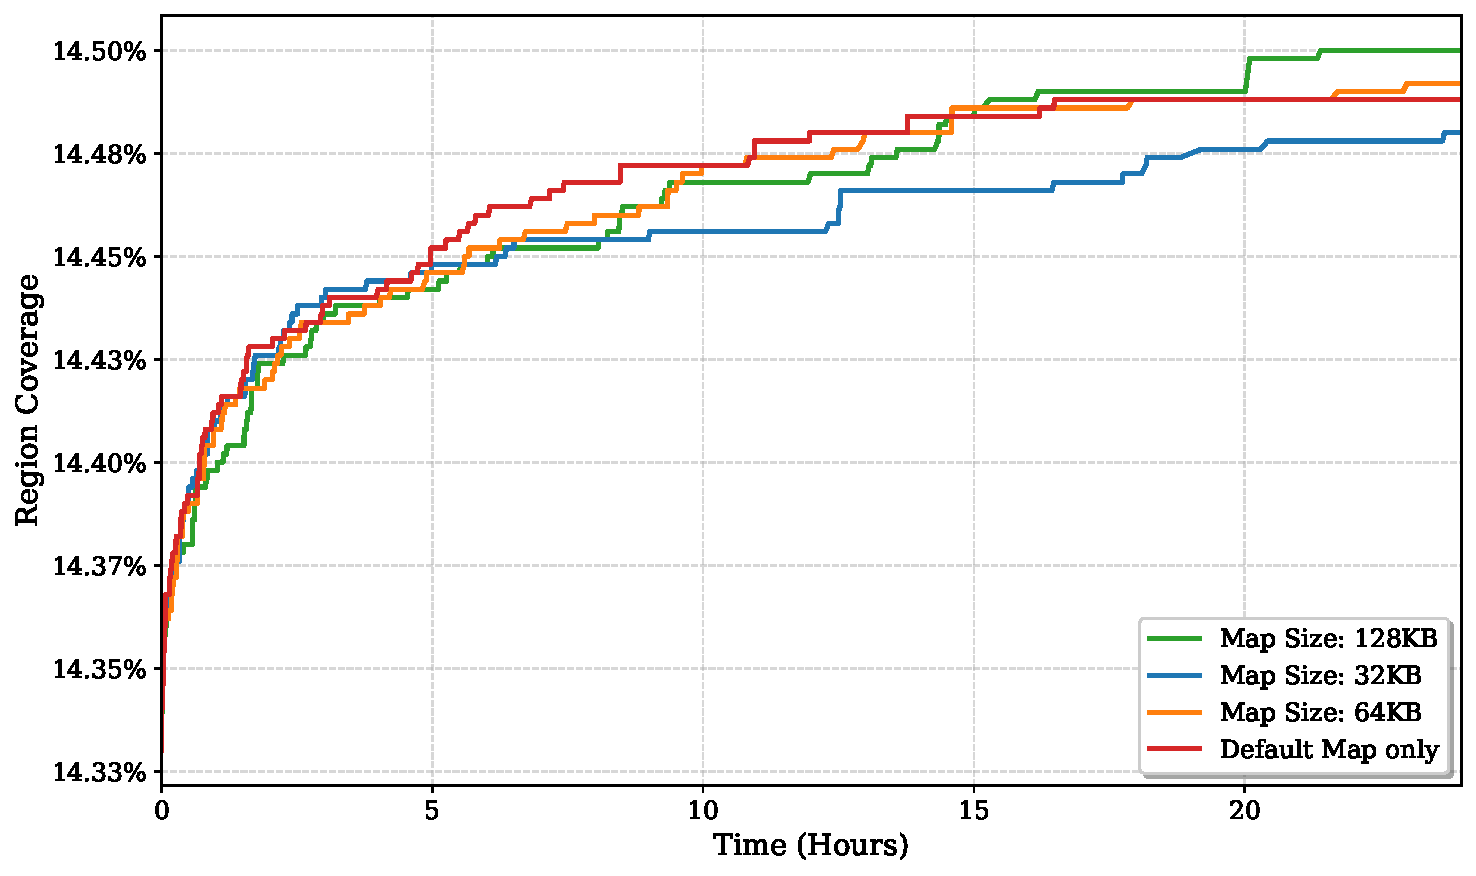
\includegraphics[width=0.85\linewidth]{imgs/eval/coverage_plot_openssl.pdf}
        \caption{OpenSSL}
        \label{fig:plot_openssl}
    \end{subfigure}

    \caption{Coverage over 24 hours for various fuzzing targets (Part 1).}
\end{figure}

% --- PAGE 2 OF THE FIGURE ---
\begin{figure}[htbp]
    \ContinuedFloat % This keeps the figure number the same
    \centering

    \begin{subfigure}{\textwidth}
        \centering
        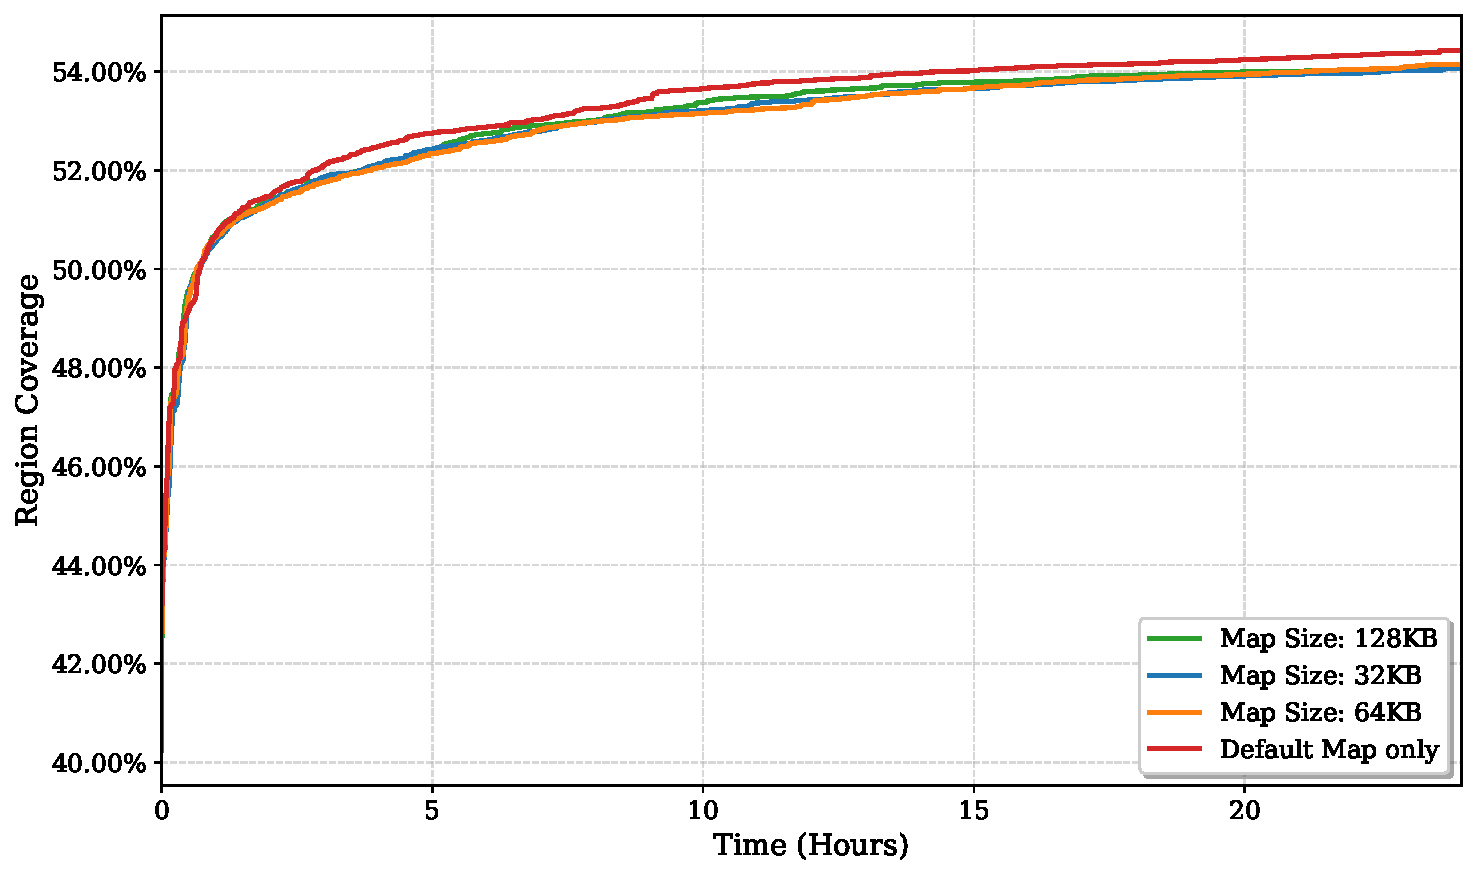
\includegraphics[width=0.85\linewidth]{imgs/eval/coverage_plot_libxslt.pdf}
        \caption{libxslt}
        \label{fig:plot_libxslt}
    \end{subfigure}
    
    \vspace{2em}

    \begin{subfigure}{\textwidth}
        \centering
        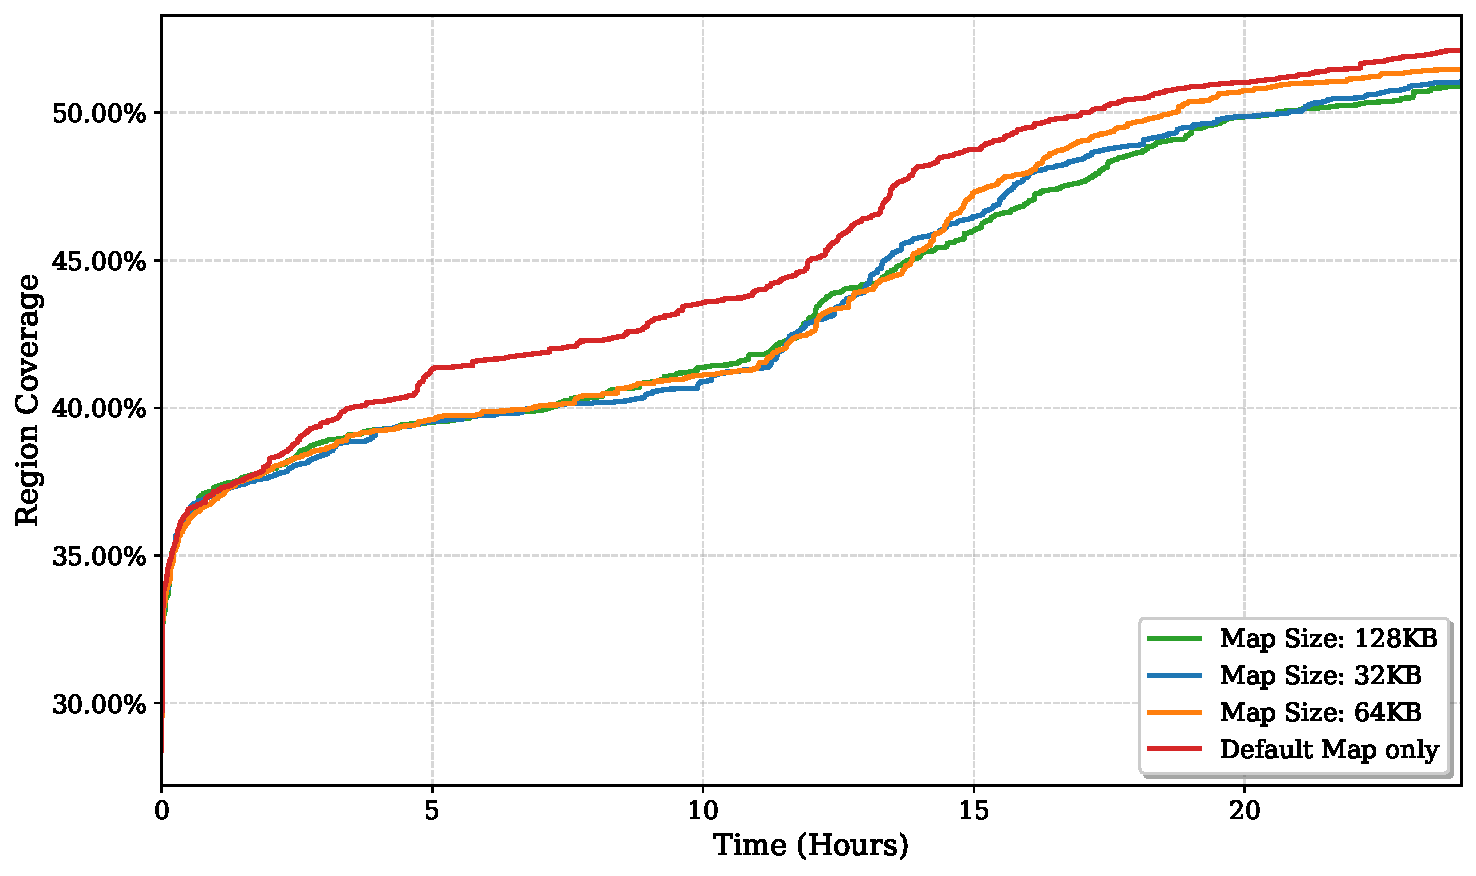
\includegraphics[width=0.85\linewidth]{imgs/eval/coverage_plot_sqlite3.pdf}
        \caption{SQLite3}
        \label{fig:plot_sqlite3}
    \end{subfigure}
    
    \caption{Coverage over 24 hours for various fuzzing targets (Part 2).}
\end{figure}


\begin{figure}[htbp]
    \ContinuedFloat % This keeps the figure number the same
    \centering

    \begin{subfigure}{\textwidth}
        \centering
        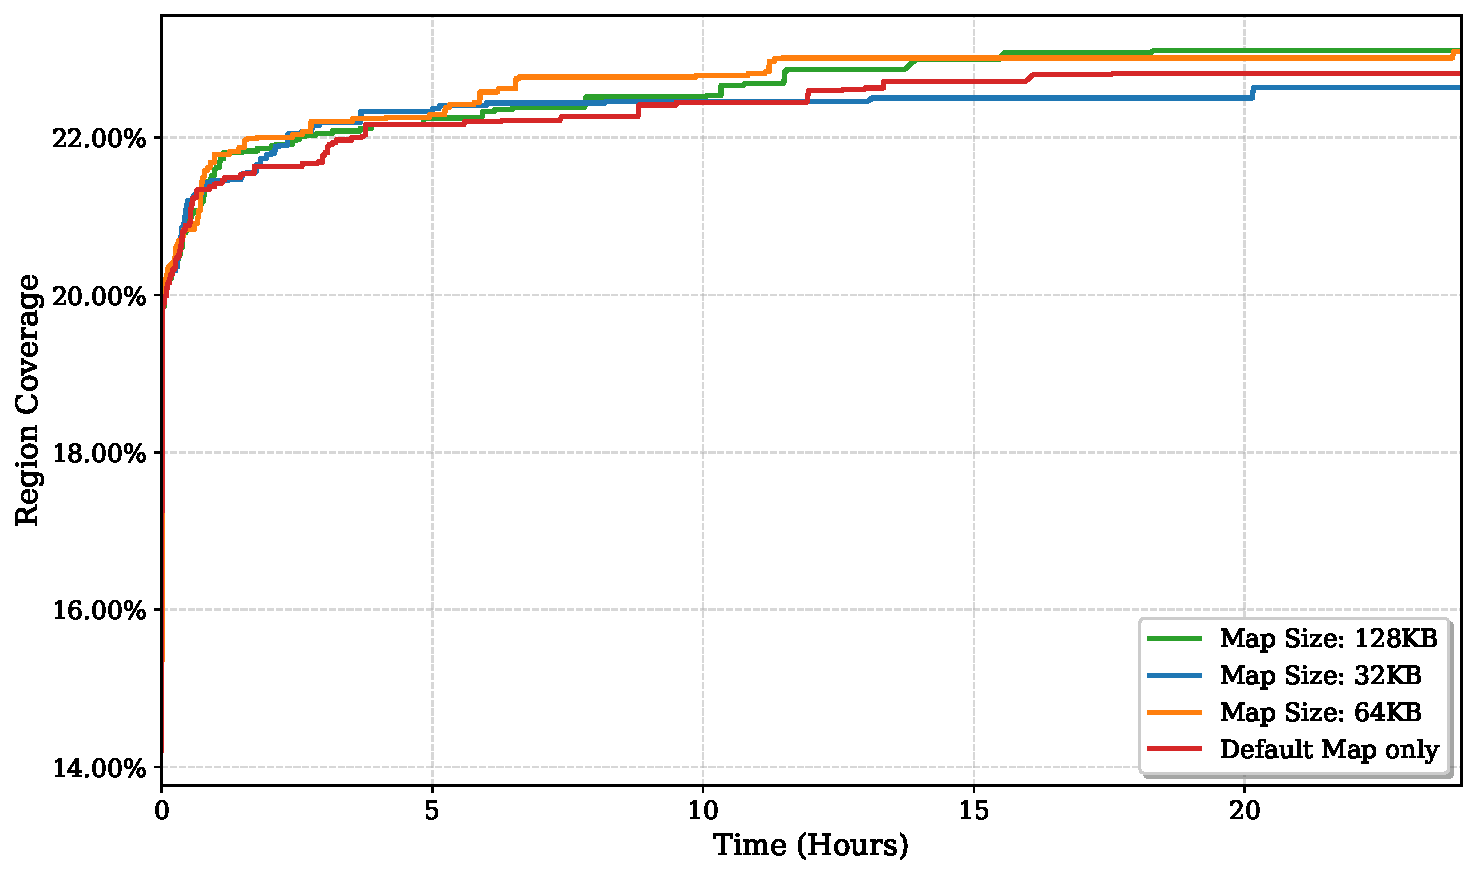
\includegraphics[width=0.85\linewidth]{imgs/eval/coverage_plot_systemd.pdf}
        \caption{systemd}
        \label{fig:plot_systemd}
    \end{subfigure}

    \caption{Coverage over 24 hours for various fuzzing targets (Part 3).}
    \label{fig:cov_plots} % The main label 
\end{figure}